\documentclass[output=paper]{langsci/langscibook}  
\ChapterDOI{10.5281/zenodo.1300632}
\author{Carmen del Río\affiliation{Universitat Pompeu Fabra}\and Maria Juan-Garau\affiliation{University of the Balearic Islands}\lastand Carmen Pérez-Vidal\affiliation{Universitat Pompeu Fabra}}
\title{Teachers’ assessment of perceived foreign accent and comprehensibility in adolescent EFL oral production in Study Abroad and Formal Instruction contexts: A mixed-method study}
\shorttitlerunninghead{Teachers’ assessment of perceived foreign accent and comprehensibility} 
\abstract{Research on second language acquisition has long been interested in analyzing different learning contexts that language learners experience when trying to improve their target languages (\citealt{CollentineFreed2004ssla}) such as formal instruction (FI), study abroad (SA), and, more recently, different types of immersion (\citealt{Pérez-Vidal2017}). The aim of the present study is to examine two of these contexts, SA and FI at home, in the case of English as a foreign language adolescent learners having Catalan and Spanish as their first languages, an age band which has received comparatively less attention than others (but see \citealt{Llanes2012,LlanesMuñoz2013}). We focus on the learners’ foreign accent and comprehensibility, as judged by a group of non-native listeners, with the objective of assessing progress and the relationship between both dimensions, following \citet{TrofimovichIsaacs2012}. Most centrally, we are interested in analyzing the aspects of each speech dimension of focus which have reportedly affected the judges’ ratings. In order to do that, speech samples were collected longitudinally for the SA (N = 25) and the FI (N = 31) groups of learners, respectively, with a pre-test/post-test design. Listeners were asked to rate and report on the aspects which affected their ratings. Our results reveal that the aspect which most influenced the judges was pronunciation. This places pronunciation at the center of the search for better practices in instructed second language acquisition in line with recently published studies (\citealt{VanLoon2002,DarcyEtAl2012,GordonDarcy2012,SaitoLyster2012,Grant2014}).}
\maketitle

\begin{document}


\section{Introduction}

Within the communicative approach to \isi{language teaching}, many second language (\isi{L2}) researchers and teachers would agree that \isi{intelligibility} is the main aim in oral communication and {L2} \isi{pronunciation} instruction, rather than a native-like \isi{accent}. Indeed, the main objective of {L2} learners in most cases is to be able to communicate and be understood, rather than \isi{accent} reduction (\citealt{PenningtonRichards1986,DerwingMunro1997,Jenkins2000,Munro2008}). The abilities linked to communication have been described on the basis of two constructs, \isi{intelligibility} and \isi{comprehensibility}. In previous studies a distinction between these two has been made (\citealt{MunroDerwing1995,MunroDerwing1999,DerwingMunro1997,DerwingMunro2009}. Intelligibility has been defined as the extent to which a given utterance is understood by a listener, and \isi{comprehensibility} has been used to refer to the listeners’ own perception of how easily they understand an utterance. However, in the present study, we have chosen the term ‘\isi{comprehensibility}’ to refer to the construct which some studies have identified as ‘\isi{intelligibility}’, in line with \citet{IsaacsTrofimovich2012}.  

All in all, both in authentic communication and in the interaction which takes place with teachers in classrooms, \isi{accentedness} may play a role which, to some extent, may eventually account for the felicitious accomplishment of interactions. This is the focus of our study, which seeks to disentagle the issue of the degree to which speech \isi{accentedness} may count more than \isi{comprehensibility} when teachers evaluate learners. More specifically, we first want to examine the correlation between these two speech dimensions based on the ratings provided by the teachers/listeners in our study  in relation to the \isi{pronunciation} of two groups of \ili{English} as a \isi{foreign language} (\isi{EFL}) adolescent learners: one group experiencing a 3-month study abroad (SA) programme, and another group experiencing \isi{conventional formal instruction} in the at home (\isi{AH}) institution. In a previous research study (\citealt{delRío2013}) we compared gains in those two dimensions by each group respectively. Results indicated that SA participants obtained significantly greater gains in \isi{FA} than the \isi{AH} group. The findings also suggested that the SA context was more beneficial than the \isi{AH} context in terms of \isi{comprehensibility} development, since the percentage of learners improving their \isi{comprehensibility} scores during SA was significantly larger than the percentage of learners improving their scores in the \isi{AH} context, and SA learners obtained larger \isi{comprehensibility} gains than \isi{AH} learners, although such improvement was not significant (see \citealt[139--164]{delRío2013}). Second, we want to explore the aspects which listeners consider when evaluating foreign \isi{accent} and \isi{comprehensibility} in SA learners’ speech samples when completing a perception task. We aim at identifying and drawing comparisons across the different factors underlying the judges’ \isi{accentedness} and \isi{comprehensibility} ratings (following the analyses conducted by \citealt{TrofimovichIsaacs2012}).  As pointed out by \citet{Isaacs2010}, knowledge of the factors influencing \isi{comprehensibility} in {L2} speech can help teachers to set instructional objectives, integrate \isi{pronunciation} with the teaching of other skills, and take these questions into account in their assessment practice in the \isi{EFL} classroom, and when preparing learners for SA experiences.


\section{Literature review}

Two main principles have traditionally led the discussion about the objectives of \isi{pronunciation} instruction: the \textit{nativeness} \textit{principle} versus the \textit{intelligibility} \textit{principle} \citep{Levis2005}, i.e. \isi{comprehensibility}. The \textit{nativeness} \textit{principle} aims at native-like \isi{pronunciation} for {L2} speakers, whereas the \textit{intelligibility} \textit{principle} considers \isi{intelligibility}. , That is, how easily messages can be understood (what we refer as \isi{comprehensibility} in this article)as the primary objective. 

Following the latter principle, most {L2} \isi{pronunciation} research does not consider \isi{accent} reduction to be the goal for communicative teaching and claims that \isi{pronunciation} teaching should aim at language \isi{intelligibility} (\citealt{Kenworthy1987,Pennington1996,Derwing2008,Thomson2013}). Thus, the interest when teaching \isi{pronunciation} is not centred on the nuances of particular speech sounds, but on getting the {L2} learners up to a level of competence which should allow them to deal with everyday communication situations \citep{Gimson1994}. 

In this study we have chosen to adopt the construt of ‘\isi{intelligibility}’ and not that of nativelikeness  in line with \citet{IsaacsTrofimovich2012}, who adopted \citeapo{Levis2006} distinction between broad and narrow definitions of \isi{intelligibility}. In its narrow sense, \isi{intelligibility} refers to listeners’ actual understanding of {L2} speech (\citealt{MunroDerwing1999}). It is often measured by examining listeners’ accuracy in providing orthographic transcriptions of {L2} speech, although other methods have also been used (e.g. comprehension questions, true-false statements, reaction times). In its broad sense, \isi{intelligibility} is defined as listeners’ ability to understand speech. 

However, the story does not end here, as two other concepts have also been the focus of attention when discussing \isi{pronunciation} in \isi{formal instruction}: \textit{foreign} \textit{accent} and \textit{comprehensibility}.  The former reflects how far from target-like standards learners’ speech is, the latter, how easy it is for listeners to perceive the information contained in learners’ messages \citep{Isaacs2010}. As far as \isi{accentedness} is concerned, we understand this concept as the listeners’ perception of how closely the \isi{pronunciation} of an {L2} utterance resembles that of a NS of \ili{English} (\citealt{MunroDerwing1995,MunroDerwing1999,DerwingMunro1997,DerwingMunro2009}. Although {L2} learners do not necessarily consider having a native-like \isi{pronunciation} as a priority, there might be {L2} learners who aim at achieving it for different reasons (e.g. professional reasons, building up a certain ‘self-image’, \isi{integrative motivation}, etc.). In contrast, we may find {L2} learners preferring to retain something of their first language (L1) \isi{accent} when speaking in an additional language (\citealt{PorterGarvin1989}). \citet[7]{DaltonSeidlhofer1994} note that “\isi{pronunciation} is so much a matter of self-image that students may prefer to keep their \isi{accent} deliberately, in order to retain their self-respect or to gain the approval of their peers.” This is indeed what we often find as teachers in the \isi{foreign language classroom} when our students tend to avoid sounding ‘\ili{English}’, since this can result in their peers joking about their ‘native like \isi{accent}’ (\citealt{FisherEvans2000}). As for \isi{comprehensibility}, according to \citet[252]{Levis2006}, \isi{intelligibility} “is not usually distinguished from closely related terms such as \isi{comprehensibility}” and has been typically measured through listeners’ ratings of how easily they understand speech (\citealt{MunroDerwing1999}). As \citet{IsaacsTrofimovich2012} pointed out, it is actually \isi{comprehensibility} (not \isi{intelligibility}) that is being assessed when listeners rate how easily they understand the information contained in a message. Therefore, in line with \citet{TrofimovichIsaacs2012}, in this study, instead of \isi{intelligibility}, we have adopted the construct of \isi{comprehensibility}, which falls under Levis’ broad sense of \isi{intelligibility} and reflects a common approach to assessing \isi{intelligibility} in oral \isi{proficiency} scales.

Finally, and most importantly for this study,  it must be pointed out that the two constructs, foreign \isi{accent} and \isi{comprehensibility}, have been claimed to constitute two partially independent dimensions. Regrettably, this may not be reflected in some assessment rubrics and actual assessment practices, which very often conflate these two different, albeit partially overlapping, dimensions of \isi{speech production}. As \citet[92]{MunroDerwing1995} note, we may find \isi{pronunciation} assessment scales ranging from “not accented, perfectly comprehensible at one endpoint to accented and difficult to understand at the other.” Given the possible overlap between different dimensions in popular assessment practices, our research study precisely aims at analyzing whether teachers are aware of these two different constructs currently included in the analysis of \isi{speech production}. In other words, the aim of this study is to examine the extent to which teachers bear in mind the distinction between foreign \isi{accent} and \isi{comprehensibility} when they rate their learners’ speech productions.

In this respect, results reported by previous studies examining the relationship between foreign \isi{accent} and \isi{comprehensibility} posit that heavily accented speech can often be perfectly understood (\citealt{MunroDerwing1995,MunroDerwing1999,DerwingMunro1997,GallardodelPuertoEtAl2007,Munro2008,Hayes-HarbWatzinger-Tharp2012}). Producing comprehensible speech is more than a matter of \isi{pronunciation}. While it is true that some errors in \isi{pronunciation} may affect speech \isi{comprehensibility}, \isi{foreign-accented speech} does not necessarily impede \isi{comprehensibility}. Thus, if \isi{comprehensibility} is the main objective of \isi{pronunciation} instruction, the degree of foreign \isi{accent} in {L2} learners’ oral productions should be of minor concern, and \isi{accent} reduction should not be a priority. Rather, those aspects of {L2} speech that appear to interfere with listeners’ comprehension of the learners’ production should be the focus. The question is: which aspects do seem to affect \isi{comprehensibility}? 

A research priority is to distinguish the aspects of {L2} speech that hinder \isi{comprehensibility} from those that, while noticeable or irritating, do not impede understanding the message (\citealt{Munro2008,IsaacsTrofimovich2012}). Little empirical research has examined the particular aspects of \isi{foreign-accented speech} which affect \isi{comprehensibility} (\citealt{MunroDerwing1995}, \citealt{MunroDerwing1999}; \citealt{Zielinski2008,IsaacsTrofimovich2012,TrofimovichIsaacs2012}). Moreover, opinions of a particular {L2} speaker’s \isi{pronunciation} problems may vary from listener to listener since familiarity with accented speech and individual differences in the ability to comprehend {L2} speech may influence foreign \isi{accent} and \isi{comprehensibility} perception (\citealt{GassVaronis1984,MunroDerwing1999}). 

In line with \citet{DerwingMunro2009}, we believe it is appropriate to work on those aspects of \isi{accent} which may affect \isi{comprehensibility}. Some studies have indicated that \isi{pronunciation} training can help {L2} speakers produce more comprehensible speech. \citet{DerwingEtAl1998} examined perceived \isi{accentedness}, \isi{comprehensibility} and \isi{fluency} in the oral productions of {L2} learners of \ili{English}. The learners were assigned to one of these conditions:
(1) no specific \isi{pronunciation} instruction group; 
(2) global instruction group, who received instruction with a focus on features such as speaking rate, \isi{intonation}, rhythm, projection, \isi{word stress}, and sentence stress; and 
(3) segmental instruction group, who received instruction to improve their production of individual sounds. Their research concluded that even though the two groups receiving instruction in \isi{pronunciation} showed significant improvement in \isi{accentedness} and \isi{comprehensibility} on the sentences, only the group receiving global instruction showed improvement in \isi{comprehensibility} and \isi{fluency} in the narratives. 

In line with these results, \citet[285]{MunroDerwing1999} reported that “prosodic errors appear to be a more potent force in the loss of \isi{intelligibility} than \isi{phonetic} errors.” These findings are in opposition with the actual situation in the \isi{EFL} classroom, where much \isi{pronunciation} practice and error correction focuses on the segmental level.

More recently, \citet{TrofimovichIsaacs2012} and \citet{IsaacsTrofimovich2012} explored the \isi{linguistic} aspects which affect foreign \isi{accent} and \isi{comprehensibility}. In the former study, \citet{TrofimovichIsaacs2012} concluded that both dimensions were related to many speech measures, but that “four categories uniquely distinguished \isi{accent} from \isi{comprehensibility}, with all categories specific to the dimension of \isi{phonology} (i.e. vowels and consonants, syllables, sounding nativelike, and rhythm)”, whereas \isi{comprehensibility} was additionally linked to \isi{grammatical} accuracy and \isi{lexical richness}. Although it is true that speaking involves \isi{pronunciation}, it is worth highlighting that {L2} speech \isi{comprehensibility} was found to be linked to vocabulary and grammar. In the second study, \citet{IsaacsTrofimovich2012} studied the construct of \isi{comprehensibility} in greater depth, and explored the aspects of speech that affected {L2} \isi{comprehensibility} at different ability levels. Based on the analyses of 19 quantitative speech measures, and listeners’ judgments and introspective reports, the authors identified five speech measures that distinguished between {L2} learners at different \isi{comprehensibility} levels: “\isi{lexical richness} and \isi{fluency} measures differentiated between low-level learners; \isi{grammatical} and discourse-level measures differentiated between high-level learners; and \isi{word stress} errors discriminated between learners of all levels” (\citealt{IsaacsTrofimovich2012}: 476). Thus, it is interesting to highlight that not only \isi{pronunciation} features of \isi{foreign-accented speech}, but also other language aspects affect speech \isi{comprehensibility} (e.g. vocabulary, grammar, and discourse measures). 

The studies mentioned above included \ili{English} native speakers (\isi{NSs}) as listeners of {L2} learners’ \isi{oral production}. It has been claimed that work on perceived \isi{accentedness} and \isi{comprehensibility} with non-native listeners is still insufficient (\citealt{DerwingMunro2011,IsaacsTrofimovich2012}). What for example some of these studies have suggested is the possibility of a speech \isi{comprehensibility} benefit in those situations where non-native speakers (\isi{NNSs}) and listeners share the same {L1} background (\citealt{GallardodelPuertoEtAl2007}). However, further evidence is necessary to strengthen this argument. Thus, the present study provides data regarding perceived foreign \isi{accent} and \isi{comprehensibility}, with data from a group of adolescent \isi{EFL} learners who have experienced a period of residence in the \isi{target language} country (United Kingdom) and \isi{formal instruction} (\isi{FI}) in their home country, Spain, and from a group of \ili{Spanish} {L1} non-native listeners, who are \isi{EFL} teachers, allowing for comparisons with previous studies including native listeners to be made to see if our results agree with previous findings. 

Concerning the specific focus of this study, there is a bulk of research  focusing on \isi{accentedness} and \isi{comprehensibility} with a similar population, namely \isi{FI} \isi{EFL} learners in Spain, sometimes contrasting them with Content and Language Integrated Learning (\isi{CLIL}) learners (\citealt{GarcíaLecumberriGallardodelPuerto2003,GallardodelPuertoEtAl2007,RalloJuan-Garau2011}). However, to our knowledge, none of them has included a group participating in a SA context of learning, and examined the possible differences which may result (but see \citealt{Llanes2012,LlanesMuñoz2012}). In sum, no previous study exists focusing on the issues of \isi{accentedness} and \isi{comprehensibility}, from the perspective of the raters, in the case of adolescent SA \isi{EFL} learners.


\section{The present study}

The current study aims at probing the constructs of foreign \isi{accent} and \isi{comprehensibility} as understood and used by listeners when asked to rate \isi{EFL} learners’ \isi{speech production}. Learners experience two different learning contexts, \isi{FI} and SA. The fact that listeners were asked to judge at the same time speech from learners who had experienced either a SA \isi{learning context} or a \isi{FI} context of learning strengthens the robustness of the data.

Our study examines a sample of oral narratives from a group of adolescent \isi{EFL} learners completing their secondary education. The speech samples were collected longitudinally before (pre-test) and after (post-test) the SA period experienced by the first group of learners, and before and after the \isi{AH} period experienced by the other group of learners, respectively. The oral productions from both groups of participants were grouped together and presented to the listeners for their evaluation in terms of perceived foreign \isi{accent} and \isi{comprehensibility} by non-native listeners. We also included speech samples collected from \isi{NSs} as baseline data to assess listeners’ ratings. 

\newpage
The main objectives of this study are: (a) to explore the relationship between the constructs of foreign \isi{accent} and \isi{comprehensibility}, and (b) to identify the aspects influencing non-native listeners’ \isi{accentedness} and \isi{comprehensibility} ratings. These objectives led us to formulate the following general \isi{research question}: In the case of a group of \isi{EFL} learners experiencing a SA period, and another group experiencing a \isi{FI} period at home, to what extent are their foreign \isi{accent} and \isi{comprehensibility} related speech dimensions when judged by non-native listeners, and which aspects do the latter take into account for their ratings? More specifically, two sub-questions were formulated to guide the analysis and discussion presented in the following sections:

\begin{enumerate}
\item 
To what extent do degree of foreign \isi{accent} and \isi{comprehensibility} correlate, in the case of a group of \isi{EFL} learners experiencing a SA period, and another group experiencing \isi{FI} period at home?
\item 
Which aspects do listeners report as affecting their foreign \isi{accent} and \isi{comprehensibility} ratings when analysed together? 

\end{enumerate}


\section{Method}

The methodological approach taken in this research study involves production and perception tasks from two different groups of participants, {L2} learners and listeners, respectively, and uses a mixed-method approach with both quantitative and qualitative data \citep{Dörnyei2007}.


\subsection{Design}


Data from an \isi{oral production} task were collected from participants at two different times over 7 months. The first data collection (T1 or pre-test) took place in May before finishing the academic year previous to a SA period, which part of the participants undertook. SA and \isi{AH} participants were tested again after their return from a 3-month SA or after an equivalent \isi{AH} period (T2 or post-test). The SA or \isi{AH} period covered the first term of the academic year (September-December). A group of \isi{NSs} of \ili{English} was also recruited to provide baseline data. 

The speech samples obtained from these three groups of participants served as the stimuli for the perception task the listeners completed. The objective of the perception task was to examine and understand perceived foreign \isi{accent} and \isi{comprehensibility} by a group of non-native listeners.


\subsection{Participants}


The participants in this study included a group of \ili{Spanish} adolescent learners of {L2} \ili{English}, some of them having experienced a period of SA (\textit{n} = 25), and the rest \isi{AH} instruction (\textit{n} = 31), hence \isi{NNSs} (\textit{n} = 56). Moreover, a group of adolescent \ili{English} \isi{NSs} (\textit{n} = 15) was also used in the perception task to provide baseline data. The total number of participants in the three speaker groups (SA, \isi{AH}, NS) was 71. Additionally, the listeners \textit{(n} \textit{=} 12) constituted one final group of \isi{NNSs}.


\subsubsection{ EFL NNS group}

The \isi{EFL} participants were 56 adolescent learners of \ili{English} who were native \ili{Spanish} speakers (40 females, 16 males). They were from Valencia, Spain, and studied at a semi-private school in this city. All of them were between 12 and 15 years old at pre-test (\textit{M}\textsubscript{age T1} = 12.96 years), and between 13 and 15 years old at post-test (\textit{M}\textsubscript{age T2} = 13.52 years). All participants had started learning \ili{English} at school in their third year of primary education (i.e. at the age of 7-8) on a 60-minute weekly basis, and had received up to 3 hours per week of subsequent \isi{EFL} instruction at school. They reported normal hearing, and none had any detectable speech disorder. Thirty-one learners were experiencing \isi{FI} during the experimental period, and 25 had joined an optional SA programme in a British or Irish school.


\subsubsection{NS group}

This group was formed by 15 \ili{English} \isi{NSs} (10 females, 5 males) attending a state school in Majorca (Spain). Two of these participants were born in England and had arrived in Majorca 5-6 years before time of testing. The rest of students in this group were early \ili{English}-\ili{Spanish} bilinguals. All speakers in this group were between 13 and 14 years old at data collection time.


\subsubsection{Listeners}

The speech samples were rated by 12 native speakers of \ili{Spanish}/\ili{Catalan} teaching \isi{EFL} in mainstream secondary education in Spain (males = 1; females = 11). They ranged in age from 29 to 46 years (\textit{M}\textsubscript{age} = 36.75). All listeners reported normal hearing. They were all \isi{EFL} mainstream secondary education instructors in Spain, who are proficient \isi{NNSs} of \ili{English}, with no specific training in phonetics, but a long-standing professional career as \isi{EFL} instructors in mainstream education. As for their \isi{linguistic} profile, seven listeners reported \ili{Spanish} as their mother tongue, four considered both \ili{Catalan} and \ili{Spanish} as their mother tongue and one listener reported that his mother tongue was \ili{Catalan}. They also reported familiarity with British and American accents, and were highly familiar with the \ili{Spanish}/\ili{Catalan}-accented speech they had to assess, as they shared the learners’ {L1} background. They were fully qualified for teaching at secondary education levels. Their \isi{EFL} teaching experience ranged from 4 to 25 years (\textit{M}\textsubscript{teaching experience} = 12.6). They rated their own knowledge of phonetics/\isi{phonology} in \ili{English} on a scale from 1 to 5, and the results indicated a mean self-rated knowledge of 3.8. The same result was obtained when they were asked to rate their own \isi{pronunciation} of \ili{English} (\textit{M} = 3.8).


\subsection{Data collection: Instruments and procedure}
\largerpage

The participants were asked to tell an oral narrative from a picture story. The speakers’ extemporaneous speech was elicited using a six-frame picture story about a bank robbery. The speakers first studied the picture story for about one minute and then were recorded individually. High quality digital recordings were made at the learners’ schools on different days. 

A short excerpt (\textit{M}\textsubscript{duration} = 20.4 seconds) was extracted from the middle-end part of each narrative. Therefore, the content of the speech samples was kept relatively consistent across speakers. The first few seconds of the excerpt were excised from the recordings by eliminating all dysfluencies (e.g. false starts) and by using natural pauses to demarcate the end of each excerpt. The preparation of speech samples for the perception task was conducted with Praat software. The excerpts from the two time periods (T1 and T2) for the SA and \isi{AH} participants, and from T0 in the case of the NS group, were then normalized for peak intensity and randomized for presentation to the listeners. This procedure is consistent with previous studies using ratings of speech samples from the same task (\citealt{Rossiter2009,TrofimovichIsaacs2012,DerwingMunro2013}). 

A total of 127 speech samples were obtained from the three groups of participants in the study. The SA  and the \isi{AH} group  recorded the story at two data collection times (56 x 2 = 112 speech samples), and the group of baseline \isi{NSs} (\textit{n} = 15) produced the speech samples once (15 speech samples).

Measures of perceived degree of foreign \isi{accent} and \isi{comprehensibility} were obtained from 12 listeners who performed a rating task. The rating task was created and presented to the listeners using the e-learning platform Moodle. The listeners read an introduction to the online rating task providing information about the context of the experiment and the procedure. They were instructed to view the cartoon story on which the oral narratives were based to minimize familiarity effects. 

Next the listeners heard the speech samples produced by the SA group (\textit{n} = 25) and the \isi{AH} group (\textit{n} = 31) at pre-test and post-test, and by the group of baseline \isi{NSs} (\textit{n} = 15), who had been recorded once. Listeners heard the 127 stimuli in randomized order and assigned ratings using separate seven-point Likert-type scales for \isi{accentedness} (1 = heavy foreign \isi{accent}, 7 = native-like \isi{accent}) and \isi{comprehensibility} (1 = extremely difficult to understand, 7 = extremely easy to understand), respectively. A 9-point scale has been most commonly used in this type of study, in which participants usually differed greatly in \isi{proficiency} level. However, a 7-point scale was deemed more appropriate for the data in the present study, taking into account the smaller degree of variability in our speech samples (SA and \isi{AH} participants with a similar age and \isi{proficiency} level), as compared to other \isi{FA} and \isi{comprehensibility} studies. As indicated in the instructions for the listeners, \isi{accentedness} was defined as how different they thought the speaker sounded from a NS of \ili{English}, if at all; and \isi{comprehensibility} as how easy or difficult the sample was to understand. Listeners were instructed to use the whole scale over the course of the experiment. In line with previous research (\citealt{DerwingMunro2013}), the mean foreign \isi{accent} scores for native participants in our research (\textit{M} = 6.71, \textit{SD} = 0.41) indicated that listeners had recognized them during the rating task, and had assigned them high scores on the 7-point rating scale. 

The listeners were also asked to comment on the aspects of speech that had influenced their \isi{comprehensibility} ratings for 20 of the speech samples, excluding the NS samples from this portion of the task. They were instructed to write their comments on the aspects of speech that they had found most striking and that they had taken into account when rating \isi{comprehensibility}. They could use bullet points and report their impressions in \ili{English}, \ili{Spanish} and/or \ili{Catalan}. Listeners were also asked to rank the top three aspects that they felt had most influenced their \isi{accentedness} ratings.

The whole rating experiment was a self-paced task. The listeners could play each speech sample as many times as needed and rate either the \isi{accentedness} or the \isi{comprehensibility} dimension first. After rating a sample, they had to click on the “Next page” button to listen to the following speech sample. Four samples were provided as rating practice at the beginning of the rating experiment so as to allow listeners to become familiar with the procedure. 

The 127 speech samples were organised in 15 parts (with 8 or 9 speech samples each). Given that this was an online rating task, listeners could pace themselves. The only restriction was that once they started whichever part of the experiment, they had to carry it out until the end. They could have a break or stop the experiment after finishing any part. 

After completing the rating experiment, the listeners were asked to summarize their listening experience by answering a short online questionnaire. The main objective of this questionnaire was to gain insight into the aspects of speech that had affected listeners’ ratings for \isi{accentedness} and \isi{comprehensibility}, the main focus of this study.

In the online questionnaire that the listeners had to complete after the rating experiment, listeners were shown a list of 12 factors and were asked to select those that had most influenced their foreign \isi{accent} and \isi{comprehensibility} ratings. They were asked to select as many as they wanted. These 12 aspects were chosen in an attempt to accommodate the various factors that can influence such ratings. In so doing, we followed \citet{KennedyTrofimovich2008}, who reported that semantic context affected listeners’ ratings for \isi{accentedness} and \isi{intelligibility}, and \citet{IsaacsTrofimovich2012}, who found that not only the \isi{pronunciation} features of \isi{foreign-accented speech}, but also other language aspects, affect speech \isi{comprehensibility} (e.g. vocaburary, grammar, and discourse measures).


\subsection{Data analysis}


Two types of analyses were conducted, quantitative and qualitative. On the one hand, the quantitative analyses measured the listeners’ ratings which were extracted from the online rating experiment and transferred to an SPSS data editor. We also examined the relationship between the participants’ degree of foreign \isi{accent} and \isi{comprehensibility}. Correlations between foreign \isi{accent} scores and \isi{comprehensibility} scores were run in order to check for the existence of a relationship between the two dimensions and its strength. 

On the other hand, the qualitative analyses dealt with the comments reported by the listeners in the online questionnaire completed after the rating experiment, stating the aspects of foreign \isi{accent} and \isi{comprehensibility} which they took into account. They sought to determine which aspects of the learners’ utterances had influenced their foreign \isi{accent} ratings and which ones had affected their \isi{comprehensibility} ratings. To gain insight into the \isi{comprehensibility} dimension, further qualitative analyses were undertaken examining the data reported by the listeners in the rating experiment on Moodle, where they were instructed to type in their comments for 20 of the speech samples.


\section{Results}

This section presents the results for the \isi{research question} and its corresponding subquestions. The main \isi{research question} addressed the strength of a potential relationship between foreign \isi{accent} and \isi{comprehensibility} when judged by non-native listeners, in the case of a group of \isi{EFL} learners experiencing a SA period, and another group experiencing a \isi{FI} period at home. The two sub-questions of the study provide the data which will allow us to address the main question and which are presented below. 


\subsection{Foreign accent and comprehensibility ratings}


In order to answer research sub-question 1, correlations between foreign \isi{accent} scores and \isi{comprehensibility} scores were run to check for the existence of a relationship between the two dimensions and its strength at the two testing times, for each of the groups examined before and after \isi{FI} and SA, respectively. A strong correlation between foreign \isi{accent} and \isi{comprehensibility} for the two groups at the two testing times was found. That is, the more native-like the \isi{accent}, the greater the \isi{comprehensibility}, both before and after \isi{FI} at home and SA (\tabref{tab:delrio:1}). 

\begin{table}
\caption{Pearson correlations between foreign accent scores and comprehensibility scores at pre-test and post-test for SA and FI groups.}
\label{tab:delrio:1}

\begin{tabularx}{.8\textwidth}{XQrr}
\lsptoprule
&  & \bfseries SA (\textit{n} = 25) & \bfseries \isi{FI} (\textit{n} = 31)\\
\midrule
\bfseries T1 & Pearson & .849 & .789\\
& Sig. & <.001 & <.001\\
\bfseries T2 & Pearson & .814 & .741\\
& Sig. & <.001 & <.001\\ 
\lspbottomrule
\end{tabularx}
\end{table}

In the following sections we examine the aspects that listeners reported as affecting their foreign \isi{accent} and \isi{comprehensibility} ratings (research sub-question 2) and explore whether listeners’ foreign \isi{accent} and \isi{comprehensibility} ratings were based on similar aspects of the learners’ oral productions.

\newpage
\subsection{Aspects influencing listeners’ foreign accent and comprehensibility ratings} 


This section tackles sub-question number 2 with the qualitative data on aspects influencing the listeners’ ratings for both foreign \isi{accent} and \isi{comprehensibility}. 


\subsubsection{Aspects influencing listeners’ foreign accent ratings}

In order to find out the aspects influencing the listeners’ \isi{accentedness} scores, and address the first part of sub-question 2, as mentioned above, listeners were given a list of 12 aspects and were asked to choose those which had most affected their foreign \isi{accent} ratings. It included the following items: grammar, vocabulary, \isi{pronunciation}, \isi{word stress}, rhythm, \isi{intonation}, repetition of words, number of filled pauses with ‘ums’ and similar items, number of silent pauses, speakers’ story telling abilities, lack of thematic content, and lack of \isi{content organization} (adapted from \citealt{IsaacsTrofimovich2012,TrofimovichIsaacs2012}). \figref{fig:delrio:1} shows the list with the 12 aspects and the raw number of listeners who selected each aspect:

\begin{figure}
\caption{\label{fig:delrio:1} Aspects affecting foreign accent ratings}
% 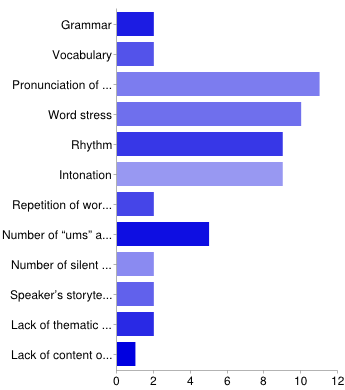
\includegraphics[width=\textwidth]{figures/delrio-img1.png} 

    \begin{tikzpicture}
        \begin{axis}[
            width  = .5\textwidth,
            height = .6\textheight,
            ylabel={},
            xlabel={}, 
            symbolic y coords={
	      Lack of content organization,
	      Lack of thematic content, 
	      Speaker's storytelling ability, 
	      Number of silent pauses, 
	      Number of ums and uhs, 
	      Repetition of words,
	      Intonation, 
	      Rhythm, 
	      Word stress, 
	      Pronunciation of vowels and consonants, 
	      Vocabulary, 
	      Grammar 
            },  
	    yticklabels={
	      Grammar, 
	      Vocabulary, 
	      Word stress, 
	      Rhythm, 
	      Pronunciation of vowels and consonants, 
	      Intonation, 
	      Repetition of words,
	      Number of \textit{ums} and \textit{uhs}, 
	      Number of silent pauses, 
	      Speaker's storytelling ability, 
	      Lack of thematic content, 
	      Lack of content organization
            },
            ytick=data,
            axis lines*=left,  
            xmin=0,
            xbar,
            bar width = 5mm,
            nodes near coords,
            nodes near coords align={horizontal},
            axis on top,
%             y dir=reverse
        ]    
        \addplot+[lsMidBlue!80!black,fill=lsMidBlue] coordinates {%
        (2,Grammar) 
        (2,Vocabulary)
        (10,Word stress) 
        (9,Rhythm) 
        (11,Pronunciation of vowels and consonants) 
        (9,Intonation) 
        (2,Repetition of words) 
        (5,Number of ums and uhs) 
        (2,Number of silent pauses)
        (2,Speaker's storytelling ability) 
        (2,Lack of thematic content) 
        (1,Lack of content organization) 
        };
%         \legend{nov, semi}
        \end{axis}
    \end{tikzpicture} 
\end{figure}
 

Factors from the domain of \isi{phonology} seemed to contribute the most to listeners’ perception of foreign \isi{accent}. Both segmental and suprasegmental aspects of speech were selected by most listeners. Pronunciation of individual sounds was selected by 92\% of the listeners, followed by \isi{word stress} (reported by 83\% of the raters), and rhythm and \isi{intonation} (75\% each). The next aspect selected by most teachers was “the number of ‘ums’ and ‘uhs’” (42\%), with a considerably lower percentage, however. 

As mentioned above, listeners were also asked to rank the top three aspects that they felt had most influenced their \isi{accentedness} ratings. As illustrated in \figref{fig:delrio:2}, the three most selected aspects influencing listeners’ foreign \isi{accent} ratings were \isi{pronunciation} of individual sounds, \isi{intonation}, \isi{word stress}, and rhythm. Other aspects which were reported by the listeners’ are shown in this figure (e.g. grammar, vocabulary, number of pauses and number of ‘uhms’ and ‘uhs’):

\begin{figure}
\caption{\label{fig:delrio:2} Aspects affecting listeners’ foreign accent ratings most (\%)}
% 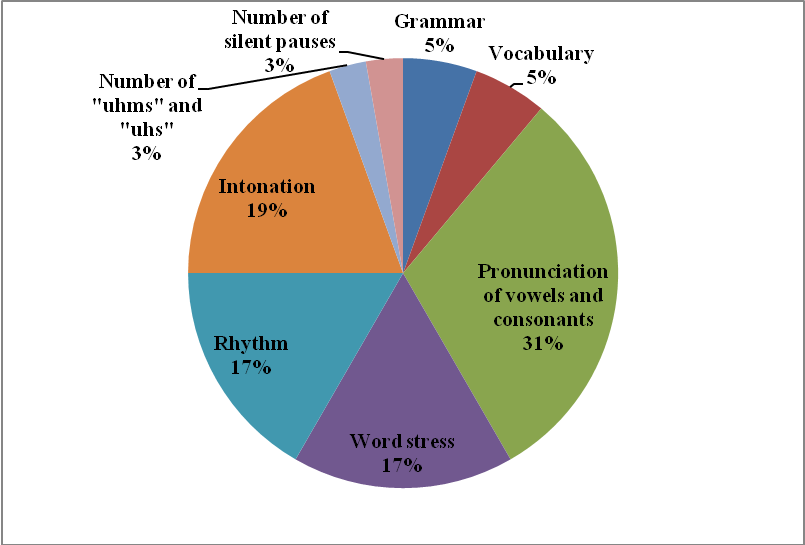
\includegraphics[width=\textwidth]{figures/delrio-img2.png}
\begin{tikzpicture}
[
    pie chart,
    slice type={intonation}{lsMidDarkBlue},
    slice type={rhythm}{lsSoftGreen}, 
    slice type={stress}{lsYellow}, 
    slice type={pronunciation}{lsLightGreen}, 
    slice type={vocabulary}{lsLightGray}, 
    slice type={grammar}{lsMidGreen},  
    slice type={pauses}{lsLightBlue}, 
    slice type={ums}{lsMidBlue},
    pie values/.style={font={\small}},
    scale=2
]
\pie{}{19/intonation,17/rhythm,17/stress,31/pronunciation,5/vocabulary,5/grammar,3/pauses,3/ums}
 \legend[shift={(2cm,17mm)}]{{Intonation}/intonation, 
 {Rhythm}/rhythm, 
 {Word stress}/stress, 
 {Pronunciation of vowels and consonants}/pronunciation, 
 {Vocabulary}/vocabulary, 
 {Grammar}/grammar,
 {Number of silent pauses}/pauses, 
 {Number of \textit{ums} and \textit{uhs}}/ums}
\end{tikzpicture}
\end{figure}
 

 
\subsubsection{Aspects influencing listeners’ comprehensibility ratings}

As regards the second part of sub-question two, that is, the analysis of the aspects influencing listeners’ \isi{comprehensibility} scores, listeners were given a list of 12 aspects and were asked to choose those which had most affected their \isi{comprehensibility} ratings. The list was identical to the one used for foreign \isi{accent} and included: grammar, vocabulary, \isi{pronunciation}, \isi{word stress}, rhythm, \isi{intonation}, repetition of words, number of filled pauses with ‘ums’ and similar items, number of silent pauses, speakers’ story telling abilities, lack of thematic content, and lack of \isi{content organization}. A summary of the results is presented in \figref{fig:delrio:3}.

\begin{figure}
\caption{\label{fig:delrio:3} Aspects affecting comprehensibility ratings}
% 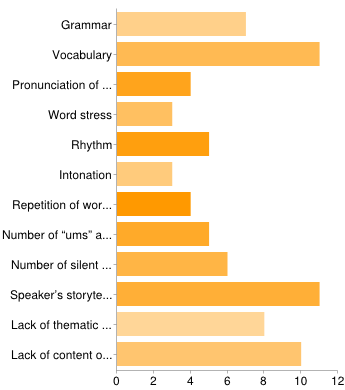
\includegraphics[width=\textwidth]{figures/delrio-img3.png}


    \begin{tikzpicture}
        \begin{axis}[
            width  = .5\textwidth,
            height = .6\textheight,
            ylabel={},
            xlabel={}, 
            symbolic y coords={
	      Lack of content organization,
	      Lack of thematic content, 
	      Speaker's storytelling ability, 
	      Number of silent pauses, 
	      Number of ums and uhs, 
	      Repetition of words,
	      Intonation, 
	      Rhythm, 
	      Word stress, 
	      Pronunciation of vowels and consonants, 
	      Vocabulary, 
	      Grammar 
            },
            ytick=data,
            axis lines*=left,  
            xmin=0,
            xbar,
            bar width = 5mm,
            nodes near coords,
            nodes near coords align={horizontal},
            axis on top,
        ]    
        \addplot+[lsMidBlue!80!black,fill=lsMidBlue] coordinates { (7,Grammar) (11,Vocabulary) (4,Pronunciation of vowels and consonants) (10,Lack of content organization) (8,Lack of thematic content) (11,Speaker's storytelling ability) (6,Number of silent pauses) (5,Number of ums and uhs)  (4,Repetition of words) (3,Intonation) (5,Rhythm) (3,Word stress) };
%         \legend{nov, semi}
        \end{axis}
    \end{tikzpicture} 
\end{figure}
 

Unlike \isi{accent}, \isi{comprehensibility} was mostly associated with vocabulary and discourse (storytelling and \isi{content organization}). More than 90\% of the listeners selected ‘vocabulary’ and ‘speaker’s storytelling ability’, and 83\% bore in mind ‘\isi{content organization}’ when assigning \isi{comprehensibility} scores. Lack of thematic content was important for 67\% of the listeners, and grammar influenced the ratings of 60\% of the listeners.

\largerpage
Seventy-five percent of these comments referred to vocabulary. Two listeners pointed out the use of {L1} vocabulary as interfering with \isi{comprehensibility}. The lack of vocabulary was stressed by one of the raters especially. Interestingly, one of the listeners highlighted that speaker’s attitude had also affected her \isi{comprehensibility} ratings. 

Listeners were also asked to rank the top three aspects that they felt had most influenced their \isi{comprehensibility} ratings. The three most cited aspects were vocabulary, lack of \isi{content organization} and speakers’ storytelling ability (followed by grammar and \isi{pronunciation} of individual sounds). \figref{fig:delrio:4} illustrates the results.

\begin{figure}
\caption{\label{fig:delrio:4} Aspects affecting listeners’ comprehensibility ratings most (\%)}
% 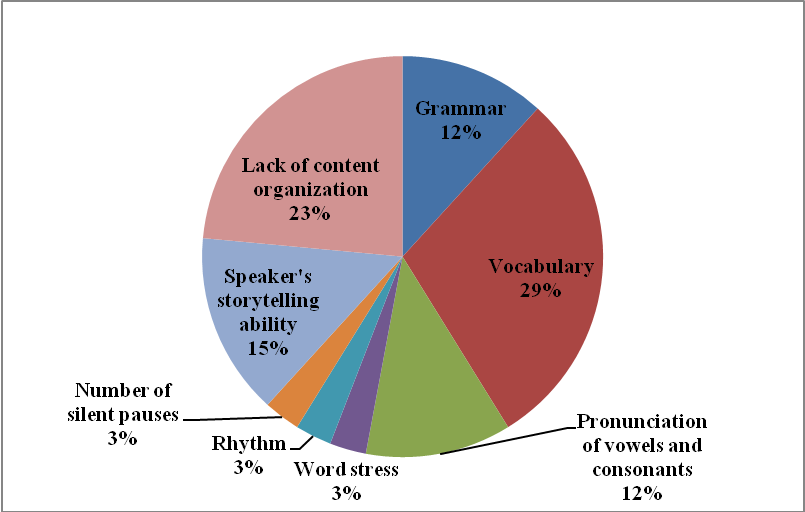
\includegraphics[width=\textwidth]{figures/delrio-img4.png}


 
    
    
\begin{tikzpicture}
[
    pie chart,
    slice type={content}{lsMidDarkBlue},
    slice type={storytelling}{lsSoftGreen},
    slice type={pauses}{lsYellow}, 
    slice type={rhythm}{lsLightGreen}, 
    slice type={stress}{lsLightGray}, 
    slice type={pronunciation}{lsMidGreen}, 
    slice type={vocabulary}{lsLightBlue}, 
    slice type={grammar}{lsMidBlue},  
    pie values/.style={font={\small}},
    scale=2
]

\pie{}{23/content,15/storytelling,3/pauses,3/rhythm,3/stress,12/pronunciation,29/vocabulary,12/grammar}

    \legend[shift={(2cm,17mm)}]{{Lack of content organization}/content, {Speaker's storytelling ability}/storytelling,  {Number of silent pauses}/pauses,  {Rhythm}/rhythm,  {Word stress}/stress,  {Pronunciation of vowels and consonants}/pronunciation,  {Vocabulary}/vocabulary,  {Grammar}/grammar}

\end{tikzpicture}
\end{figure}
 

In order to delve into the \isi{comprehensibility} construct, we asked listeners to type in their comments immediately after rating the \isi{comprehensibility} of 20 speech samples scattered throughout the rating experiment.  We obtained 688 comments about \isi{comprehensibility} from the text entry boxes which were filled in by the listeners during the rating experiment. The listeners’ descriptive comments were first classified as \textit{indicating} \textit{a} \textit{postive} \textit{or} \textit{negative} \textit{remark} \textit{on} \textit{the} \textit{comprehensibility} \textit{of} \textit{the} \textit{sample} .  There were 426 negative comments and 262 positive comments. Then the comments were thematically coded, and re-coded to eliminate overlapping ones (e.g. ‘L1 word’, ‘invented word’ and ‘wrong word’ were combined under a ‘vocabulary’ category). 

We found that some listeners were more specific than others regarding their comments. Whereas some listeners made general comments about \isi{comprehensibility} such as “grammar errors,” other listeners specified in their reports the type of grammar errors they found in the participants’ speech (e.g. “no subject,” “wrong verb tense,” etc.). \tabref{tab:delrio:2} shows all the categories obtained from the listeners’ comments indicating whether they were considered as negative (N), or positive (P) evaluations, or both (B). The initial number of comments is provided together with the final number of comments obtained, once double references to the same category made by the same listener were identified (number of comments deleted are indicated in brackets). The percentage of each category over the total number of final comments is indicated in the \% column.

\begin{table}
\caption{Frequency of coded categories for comprehensibility from teacher reports (initial raw number, final raw number, and \%)}
\label{tab:delrio:2}
\small
\begin{tabularx}{\textwidth}{l@{}SSSr}
\lsptoprule
\bfseries Category & \bfseries Considered as negative, positive or both & \bfseries Initial number of comments & \bfseries Final number of comments after re-coding & \bfseries \%\\
\midrule
Ambiguous\footnote{ There were a number of comments which were categorized as ‘Ambiguous’. They were included in this category when it was not clear what the listeners were considering. For instance, for comments such as “I can't understand some words," it was not clear whether there was a \isi{pronunciation} problem on the part of the speaker or if the speaker had invented a word which the listener could not understand (vocabulary). Given that we were not sure  whether this was a comment referring to \isi{pronunciation} or vocabulary, we assigned it to the ‘Ambiguous’ category.\textsuperscript{2} The data collection procedure comprised 3 academic years since data was collected from two consecutive cohorts of students at the same home institution.\textsuperscript{3} Data from \isi{NSs} was collected by researchers at the \textit{Universitat} \textit{de} \textit{les} \textit{Illes} \textit{Balears} participating in the SALA and COLE research projects, coordinated by \textit{Universitat} \textit{Pompeu} \textit{Fabra} (Barcelona, Spain).} & B & 10 & 10 & 1.67\\
Attitude & B & 19  (-3) & 16 & 2.68\\
Listener’s teaching profile & P & 2 & 2 & 0.33\\
Communicative strategies & B & 10 & 10 & 1.67\\
Content & B & 37  (-1) & 36 & 6.04\\
Discourse & B & 61  (-12) & 49 & 8.22\\
\ili{English} \isi{proficiency} & N & 1 & 1 & 0.16\\
Familiarity with the story & P & 4 & 4 & 0.67\\
\textbf{Fluency} & \textbf{B} & 97  (-11) & 86 & \textbf{14.42}\\
\textbf{Grammar} & \textbf{B} & 99  (-12) & 87 & \textbf{14.59}\\
L1 familiarity & B & 16  (-2) & 14 & 2.34\\
L1 influence (general comment) & N & 3 & 3 & 0.50\\
Listener’s attitude & P & 4 & 4 & 0.67\\
Low voice & N & 3 & 3 & 0.50\\
\textbf{Pronunciation} & \textbf{B} & 194   (-39) & 155 & \textbf{26}\\
Self-correction & P & 4 & 4 & 0.67\\
Style & B & 3    (-1) & 2 & 0.33\\
\textbf{Vocabulary} & \textbf{B} & 121   (-11) & 110 & \textbf{18.45}\\
\lspbottomrule
\end{tabularx} 
\end{table}

\newpage 
As can be observed, 26\% of the comments referred to \isi{pronunciation} (including segmental and supra-segmental aspects). Vocabulary was the second most frequent aspect considered by listeners in their comments (18.45\%), followed by grammar (14.59\%) and \isi{fluency} (14.42\%).  

Further analyses explored whether the above-mentioned aspects were also taken into account to a similar extent in negative and positive \isi{comprehensibility} ratings. Therefore, we examined the 426 negative comments and the 262 positive ones separately.

As for the comments identifying negative evaluations of \isi{comprehensibility}, \isi{pronunciation}, vocabulary and grammar were reported as the categories that most frequently affected listeners’ scoring decisions. Twenty-six percent of the comments referred to segmental and supra-segmental aspects of participants’ speech, 22.71\% dealt with vocabulary items, and 19.11\% with grammar. Fluency was mentioned in almost 15\% of the comments. \tabref{tab:delrio:3} shows the results of this analysis.

\begin{table}
\caption{Frequency of coded categories for negative comments on comprehensibility from teacher reports (initial raw number, final raw number, and \%).}
\label{tab:delrio:3}
\begin{tabularx}{\textwidth}{lSSr}
\lsptoprule
\bfseries Category & \bfseries Initial number of comments & \bfseries Final number of comments & \bfseries \%\\
\midrule
Ambiguous & 7 & 7 & 1.93\\
Attitude & 10 & 8 & 2.21\\
Communicative strategies & 1 & 1 & 0.27\\
Content & 19 & 19 & 5.26\\
Discourse & 20 & 19 & 5.26\\
\ili{English} \isi{proficiency} & 1 & 1 & 0.27\\
\textbf{Fluency} & 62 & 53 & \textbf{14.68}\\
\textbf{Grammar} & 80 & 69 & \textbf{19.11}\\
(No) {L1} familiarity & 3 & 1 & 0.27\\
L1 influence (general comment) & 3 & 3 & 0.83\\
Low voice & 1 & 3 & 0.83\\
\textbf{Pronunciation} & 126 & 94 & \textbf{26.03}\\
Style & 2 & 1 & 0.27\\
\textbf{Vocabulary} & 91 & 82 & \textbf{22.71}\\
\midrule
\textbf{Total} & 426 & 361 & \\
\lspbottomrule
\end{tabularx}
\end{table}

To have a better idea of the \isi{pronunciation} features, we classified the comments according to the aspect of speech they were more specifically referring to. \tabref{tab:delrio:4} shows this classification and the percentage of comments assigned to each \isi{pronunciation} category.

\begin{table}[t]
\caption{Pronunciation aspects reported by listeners as negatively influencing their comprehensibility ratings of participants’ speech}
\label{tab:delrio:4}

\begin{tabularx}{\textwidth}{Qr}
\lsptoprule

\bfseries Pronunciation aspect & \bfseries \%\\
\midrule
Pronunciation of individual sounds and words & 55.55\\
Foreign \isi{accent} & 17.46\\
Intonation & 11.11\\
Rhythm & 3.96\\
Stress & 2.3\\
Native-like \isi{pronunciation} & 4\\
Other\footnote{Comments regarding \isi{pronunciation} in general and speech clarity were categorized under the ‘Other’ category.} & 5.55\\
\lspbottomrule
\end{tabularx}
\end{table}

Half of the comments regarding \isi{pronunciation} problems referred to the \isi{pronunciation} of individual sounds or words. It is worth remarking that specific reference was made to \isi{foreign-accented speech} as an aspect affecting \isi{comprehensibility} (17\% of the comments referred to foreign \isi{accent}). However, ‘L1 interference’ was mentioned when considering other \isi{pronunciation} factors such as \isi{pronunciation} of individual sounds or words, and \isi{intonation}. Comments such as “\ili{Spanish} \isi{intonation},” “L1 influence on \isi{pronunciation}” and “typical \isi{pronunciation} mistake (from their L1)” were collected.

Having a native-like \isi{pronunciation} was regarded as hindering \isi{comprehensibility} to some extent by some of the listeners when rating native participants’ speech. Comments such as those in \REF{ex:delrio:1} were collected from listeners’ evaluations: 

\ea\label{ex:delrio:1}
EMLE: “after listening to so many recordings with the same type of syllable-timed speech, it was hard to readjust my ear to connected speech”~
\z

As regards the comments referring to aspects positively affecting \isi{comprehensibility} ratings, \isi{pronunciation} was also considered the most influential aspect. As shown in \tabref{tab:delrio:5}, \isi{fluency}, discourse and vocabulary were aspects reported in more than 10\% of the comments.

\begin{table}
\caption{Frequency of coded categories for positive comments on comprehensibility from teacher reports (initial raw number, final raw number, and \%)}
\label{tab:delrio:5}

\begin{tabularx}{\textwidth}{lSSr}
\lsptoprule
\bfseries Category & \bfseries Initial number of comments & \bfseries Final number of comments & \bfseries \%\\
\midrule
Ambiguous & 3 & 3 & 1.23\\
Attitude & 9 & 8 & 3.29\\
Being a teacher & 2 & 2 & 0.82\\
Communicative strategies & 9 & 9 & 3.70\\
Content & 18 & 17 & 7\\
\textbf{Discourse} & 41 & 31 & \textbf{12.75}\\
Familiarity with the story & 4 & 4 & 1.64\\
\textbf{Fluency} & 35 & 34 & \textbf{14}\\
Grammar & 19 & 19 & 7.81\\
L1 familiarity & 15 & 13 & 5.34\\
Listener’s attitude & 4 & 4 & 1.64\\
\textbf{Pronunciation} & 68 & 63 & \textbf{26.33}\\
Self-correction & 4 & 4 & 1.64\\
Style & 1 & 1 & 0.41\\
\textbf{Vocabulary} & 30 & 30 & \textbf{12.34}\\
\midrule 
Total & 262 & 242 & \\
\lspbottomrule
\end{tabularx}
\end{table}

As with the \isi{pronunciation} comments identifying negative aspects of participants’ speech \isi{comprehensibility}, we analyzed listeners’ reports on positive evaluations in further depth and found that listeners did not identify any particular aspects of \isi{pronunciation} as positively affecting their \isi{comprehensibility} ratings, but rather they referred to \isi{pronunciation} in general. About 40\% of the comments were similar to the following ones: “quite good \isi{pronunciation} that facilitates \isi{comprehensibility},” “\isi{pronunciation} is OK,” and “\isi{pronunciation} is not that bad”. Having a native-like \isi{pronunciation} or imitating native-like \isi{pronunciation} was the second most frequently cited aspect (22\% of the comments). Moreover, general comments on \isi{accent} were reported in 15\% of the listeners’ comments (e.g. “good \isi{accent}”). \tabref{tab:delrio:6} shows the percentage of comments assigned to each \isi{pronunciation} aspect reported by the listeners as positively affecting their \isi{comprehensibility} ratings.

\begin{table}
\caption{Pronunciation aspects reported by listeners as positively influencing their comprehensibility ratings of participants’ speech}
\label{tab:delrio:6}

\begin{tabularx}{\textwidth}{Qr}
\lsptoprule
\bfseries Pronunciation aspect & \bfseries \%\\
\midrule 
Pronunciation of individual sounds and words & 2.94\\
Accent (general comment) & 14.7\\
Intonation & 10.29\\
Rhythm & 7.35\\
Pronunciation (general positive comment) & 41.17\\
Native or imitating native-like \isi{pronunciation} & 22.05\\
Being familiar with {L1} \isi{accent} & 1.47 \\
\lspbottomrule
\end{tabularx}
\end{table}

\newpage 
While language aspects such as \isi{pronunciation}, vocabulary, grammar or \isi{fluency} were most frequently reported by listeners as affecting \isi{comprehensibility}, other aspects were mentioned which will be discussed in more detail in the following section. Reference to a NS model or the importance of native-like speech, {L1} familiarity and the speaker’s and listener’s attitude were points made by the listeners which will also receive special attention in the next pages so as to provide further answers and comments in the context of \ili{English} \isi{pronunciation} teaching today.


\section{Discussion}

The main \isi{research question} in this study enquired as to whether or not and to what extent foreign \isi{accent} and \isi{comprehensibility} are related speech dimensions when judged by non-native listeners, in the case of a group of \isi{EFL} learners experiencing a SA period, and another group experiencing a \isi{FI} period at home, and what aspects affected their decisions. 

Our results have revealed significant strong positive correlations between the two speech dimensions at the two testing times, that is before and after both \isi{FI} and SA, for both groups of participants, indicating that the more native-like the \isi{accent}, the greater the \isi{comprehensibility}, and vice-versa. These results contrast with those reported in previous studies positing that heavily accented speech can often be perfectly intelligible, which, in contrast had mostly naïve (that is, non-language professionals) \isi{NSs} as listeners (\citealt{MunroDerwing1995,MunroDerwing1999,DerwingMunro1997,GallardodelPuertoEtAl2007,Hayes-HarbWatzinger-Tharp2012}). One possible interpretation of these findings is that the sample is rather homogeneous, both in the speakers and in the listeners: The learners who provided the speech samples have been attending the same \isi{FI} class during their former education prior to data collection, and the listeners are non-native \isi{EFL} teachers, who train their students to try and achieve native-like standards. For them, \isi{accent} may actually indeed interfere with comprehension. Another interesting result was the fact that none of the participants were assigned a high foreign \isi{accent} rating and a low \isi{comprehensibility} score. In other words, participants who were assigned high \isi{comprehensibility} scores were also given good ratings in foreign \isi{accent}.

Given these three results – that is, 
(1) positive correlations between foreign \isi{accent} and \isi{comprehensibility}, 
(2) learners’ approximation to native-like \isi{accent} always associated with good \isi{comprehensibility} ratings, and (3) a contrast with the extant literature regarding the link established by listeners between \isi{accent} and \isi{comprehensibility} – our sub-question 2, which taps into the aspects which influenced listeners’ foreign \isi{accent} and \isi{comprehensibility} ratings, gained more relevance. Qualitative analyses were thus conducted of listeners’ comments gathered from the questionnaires they completed after finishing the rating task, and from 20 reports which were typed in at the same time that they provided their ratings during the rating task. 

Concerning the aspects affecting foreign \isi{accent} ratings, factors from the domain of \isi{phonology} were selected from the list by most listeners (see \figref{fig:delrio:1}). Pronunciation of vowels/consonants, \isi{word stress}, rhythm and \isi{intonation} were reported in this order as mainly affecting their foreign \isi{accent} assessment. This finding was confirmed when listeners were asked which three aspects had influenced their foreign \isi{accent} ratings most (see \figref{fig:delrio:2}). Pronunciation of vowels/consonants, \isi{intonation}, \isi{word stress} and rhythm were considered in this order. In fact, these \isi{phonological} dimensions altogether represented 84\% of the factors selected by the listeners as mostly influencing their foreign \isi{accent} ratings. These results confirmed the findings in \citet{TrofimovichIsaacs2012} indicating that \isi{accent} was mainly associated with aspects of \isi{phonology} (e.g. rhythm, segmental accuracy, and syllable structure).

On the other hand, \isi{comprehensibility} was mostly related to vocabulary and discourse aspects, such as storytelling and \isi{content organization} (see \figref{fig:delrio:3}). Lack of thematic content and grammar were also selected by more than half of the listeners. When asked to identify the three most influential aspects on their \isi{comprehensibility} ratings (\figref{fig:delrio:4}), vocabulary (29\%), lack of \isi{content organization} (23\%) and speaker’s storytelling ability (15\%) were reported in this order, followed by grammar (12\%) and \isi{pronunciation} of individual sounds (12\%). 

\newpage 
If we now consider the last part of sub-question 2, which tapped into whether listeners’ foreign \isi{accent} and \isi{comprehensibility} ratings were based on similar aspects of the learners’ oral productions, it is worth noting that even though none of the \isi{phonological} factors were as important individually for the \isi{comprehensibility} ratings as in the case of the foreign \isi{accent} ratings, \isi{pronunciation} of vowels and consonants represented 12\% of the comments, \isi{word stress} 3\% and rhythm 3\%. All these \isi{phonological} factors taken together represented 18\% of the comments related to \isi{comprehensibility} ratings, a higher percentage than, for instance, speaker’s storytelling ability, which was ranked third in the list presented above of the most influential factors affecting listeners’ assessment of \isi{comprehensibility}. 

These results are in line with \citeapo{TrofimovichIsaacs2012} findings, which indicated that \isi{comprehensibility} was mainly linked to \isi{grammatical} accuracy and \isi{lexical richness}. As seen in the literature review, \citet{TrofimovichIsaacs2012} identified five speech aspects which differentiated between {L2} learners at different \isi{comprehensibility} levels: \isi{lexical richness} and \isi{fluency} distinguished between low-level learners, \isi{grammatical} and discourse-level measures differentiated between high-level learners, and \isi{word stress} errors discriminated between learners of all levels. Overall, results in our study suggest that listeners regarded vocabulary and also discourse aspects (lack of \isi{content organization} and speaker’s storytelling ability) as the most important factors related to \isi{comprehensibility}, factors which were also indicated in  \citeapo{TrofimovichIsaacs2012} research. However, findings in our research do not support Trofimovich \& Isaacs’ conclusion pointing out that “four categories uniquely distinguished \isi{accent} from \isi{comprehensibility}, with all categories specific to the dimension of \isi{phonology} (i.e. vowels and consonants, syllables, sounding native-like, and rhythm)” (p. 912).   As we have seen, \isi{pronunciation} aspects (e.g. \isi{pronunciation} of individual sounds) were also taken into account by the listeners in our study when assessing \isi{comprehensibility}. As suggested above, the differences in listeners’ profiles in both studies, non-native language specialists in the current study versus naïve \isi{NSs} in prior works, might be the reason for this discrepancy. 

It is worth mentioning other aspects (different from the ones provided in the list) which some of the listeners reported as having influenced their \isi{comprehensibility} ratings. Almost all comments referred to vocabulary, and some of them stressed the use of {L1} items as hampering \isi{comprehensibility}, as in  
\REF{ex:delrio:2} and \REF{ex:delrio:3}. 

\largerpage[2]
\ea\label{ex:delrio:2}
INCA: “Use of \ili{Spanish} words maybe”\footnote{L1 lexical interference was confirmed to negatively affect INCA’s \isi{comprehensibility} ratings, as she reported other comments throughout the perception task such as, “use of words translated from \ili{Spanish} (‘senior’, from \ili{Spanish} word “señor” -meaning ‘man’).}. \\
\z

\clearpage 
\ea\label{ex:delrio:3}
MOLO: “The use of {L1} words in some cases which shows the lack of ability of the student to make the message be understood”
\z

The fact that these listeners considered the use and transfer of {L1} words as negatively affecting \isi{comprehensibility} does not necessarily contradict findings in previous studies suggesting the speech \isi{comprehensibility} benefit for \isi{NNSs} and non-native listeners sharing the same {L1} background (\citealt{Hayes-HarbEtAl2008,GallardodelPuertoEtAl2009}), mentioned previously. However, the analysis of all the comments gathered from listeners, including those in \REF{ex:delrio:4}--\REF{ex:delrio:6}, showed that {L1} lexical interference was not positively considered in many instances.

\ea\label{ex:delrio:4}
COGA: “The use of \ili{Spanish} words makes it confusing.”
\z

\ea\label{ex:delrio:5}
INCA: “Usa vocabulario ‘traducido’ de la lengua materna.” (‘\textit{He} \textit{“translates”} \textit{words} \textit{from} \textit{his} \textit{L1}.’) 
\z

\ea\label{ex:delrio:6}
MAGU: “Clara influencia de la lengua materna. Adapta claramente vocabulario al inglés. Es dificil de comprender por el vocabulario.” (‘\textit{Clear} \textit{influence} \textit{of} \textit{his} \textit{L1.} \textit{He} \textit{adapts} \textit{lexical} \textit{items} \textit{from} \textit{his} \textit{L1.} \textit{It’s} \textit{difficult} \textit{to} \textit{understand} \textit{because} \textit{of} \textit{the} \textit{vocabulary}.’)
\z

So far, our results partly support those reported by recent research indicating that foreign \isi{accent} and \isi{comprehensibility} are linked to different language aspects. On the one hand, we can conclude that aspects of \isi{phonology} affected foreign \isi{accent} ratings more than aspects related to other domains such as grammar or vocabulary. On the other hand, although results confirmed that vocabulary and discourse factors, as well as grammar, were the main contributors to variation in \isi{comprehensibility} ratings, reports from the listeners in our study suggested that factors related to \isi{pronunciation} also had some influence on their assessment of \isi{comprehensibility}, when considering the data from the two learning contexts together. 

The listeners were also asked to type in the aspects of speech which they were taking into account when providing their \isi{comprehensibility} ratings. Responses for 20 of the speech samples were analyzed. The analyses of these comments helped us to elucidate whether \isi{pronunciation} was actually involved (or not) in listeners' \isi{comprehensibility} ratings. 

When analyzing all the comments provided by the listeners we found that 26\% of the comments regarding their \isi{comprehensibility} ratings considered aspects of \isi{pronunciation}, 18.45\% of the comments referred to vocabulary, 14.59\% to grammar, and 14.42\% to \isi{fluency}. Therefore, a new distribution of the aspects affecting this speech dimension was obtained (compared to the 12-item classification from the final questionnaires presented above). Vocabulary was considered a key aspect for \isi{comprehensibility} in many of the comments, but \isi{pronunciation} was even more frequently highlighted. 

The comments from the reports were classified as affecting negatively or positively the listeners’ ratings. With regard to the aspects hindering \isi{comprehensibility}, 26\% of the comments were related to \isi{pronunciation}, 22.71\% associated with vocabulary, and 19\% linked to grammar. Pronunciation was also regarded as the variable enhancing \isi{comprehensibility} most. Twenty-six percent of the comments providing reasons for good \isi{comprehensibility} had to do with \isi{pronunciation}, 14\% were related to \isi{fluency}, 12.75\% to discourse, and 12.34\% were associated with vocabulary. 

Therefore, according to these analyses, \isi{comprehensibility} was related to \isi{pronunciation} to a considerable degree. In order to gain a better understanding of the \isi{pronunciation} aspects promoting (or hampering) \isi{comprehensibility}, we classified the comments according to the \isi{pronunciation} features which the listeners were particularly referring to. The top three \isi{pronunciation} features which were mentioned in negative evaluations of \isi{comprehensibility} were \isi{pronunciation} of individual sounds and words (55.5\%), foreign \isi{accent} (17.42\%), and \isi{intonation} (11.1\%). As for the \isi{pronunciation} aspects which were identified in positive comments on \isi{comprehensibility}, listeners cited \isi{pronunciation} in general (41.1\%), imitation of native-like \isi{pronunciation} (22\%), and degree of \isi{accentedness} (14.7\%), followed by \isi{intonation} (10.29\%).

\largerpage
Therefore, according to the reports on \isi{comprehensibility} provided by the listeners while carrying out the perception task, \isi{pronunciation} was found to be the most relevant aspect in their assessment of \isi{comprehensibility} of {L2} learners' speech.  The fact that \isi{pronunciation} was not ranked within the top three aspects affecting \isi{comprehensibility} in the data obtained from the questionnaires may potentially be explained in two ways. First, since we presented the questions about the factors influencing foreign \isi{accent} and \isi{comprehensibility} ratings in the same questionnaire, we could have implicitly motivated the distinction between the two constructs. Second, as already remarked, while it is true that specific \isi{pronunciation} features (e.g. \isi{pronunciation} of individual sounds, \isi{intonation}, stress, etc.) did not greatly affect \isi{comprehensibility} when considered separately, \isi{pronunciation} aspects taken as a whole did have a considerable impact on the listeners’ comments. On the other hand, we may consider the comments made by the listeners during the rating experiment as more reliable and ecologically valid than the comments collected at the end of the experiment, as the former were reported when listeners were actually rating the speech samples for \isi{comprehensibility}. 

According to these data, non-native listeners in our study took into account \isi{pronunciation} aspects when assessing {L2} learners’ \isi{comprehensibility} of \ili{English}, both after \isi{FI} and SA. First, strong positive correlations between foreign \isi{accent} and \isi{comprehensibility} were found for data from both contexts, in spite of the fact that these contexts might have affected learners differently. Second, listeners in our study did pay attention to aspects related to \isi{accent} or native-like \isi{pronunciation} when providing their \isi{comprehensibility} ratings with data from both contexts, in contrast with previous research involving native listeners of \ili{English} (\citealt{TrofimovichIsaacs2012}). Against such backdrop, further research is needed to gain a better understanding of the aspects affecting \isi{comprehensibility} as reported by native and non-native listeners.


\section{Conclusion}

In this research study we have examined foreign \isi{accent} and \isi{comprehensibility} ratings assigned by \ili{English} non-native instructors, who are frequently responsible for teaching \isi{FI} \isi{EFL} courses in the \isi{AH} context in Spain, so as to determine the relationship between these two speech dimensions, in the case of a group of \isi{EFL} learners experiencing a SA period, and another group experiencing a \isi{FI} period at home. Contrary to previous findings (\citealt{MunroDerwing1999,DerwingMunro2009}), a strong correlation has been found between foreign \isi{accent} and \isi{comprehensibility}, indicating that those learners with better \isi{accent} obtained higher \isi{comprehensibility} ratings, and learners with heavier foreign \isi{accent} were also perceived as less comprehensible. Furthermore, we have explored the aspects that listeners took into account when assessing foreign \isi{accent} and \isi{comprehensibility}. Results showed that the foreign \isi{accent} dimension was mainly associated with \isi{pronunciation} aspects, which also affected \isi{comprehensibility} ratings assigned by the non-native listeners in our research. Confirming previous research (\citealt{TrofimovichIsaacs2012}), aspects such as vocabulary and grammar were taken into account when rating {L2} learners’ speech \isi{comprehensibility} but, contrary to previous findings in studies involving native listeners of \ili{English}, \isi{pronunciation} was the aspect that listeners heeded most when assigning \isi{comprehensibility} scores. 

It remains unclear whether the aspects reported by the group of non-native listeners of our study are specific to our participants, or can be generalized to learners from different {L1} backgrounds, or experiencing other learning contexts besides \isi{FI} and SA, such as, for example, \isi{immersion} classrooms. In addition, it would be advisable to validate our findings with \ili{English} native and non-native listeners from other {L1} backgrounds and profiles. Likewise, when considering the 12 factors that influence foreign \isi{accent} and \isi{comprehensibility} ratings the most, the preponderance of aspects that concern phonetics should guide our analyses in future, paired with a more careful weighting of the factors included in the list. In these respects further research is necessary to throw more light on this area of \isi{speech production} abilities, in the case of \isi{EFL} adolescent learners. 

One of the findings in our study is the difference between ratings given by listeners who are language specialists, sharing their {L1} with the learners’ whose samples they are rating, as opposed to naïve \isi{NSs}. More research seems necessary in order to add further evidence to allow us to disentangle those two variables which now seem to be conflated and tackle the issue of listerners’ profile under this new light. Finally, although it is widely accepted that the objective of {L2} \isi{pronunciation} teaching should be to help {L2} learners be understandable for their interlocutors, classroom teachers have received little guidance on the \isi{pronunciation} features on which they should focus during lessons (\citealt{DerwingMunro2009}). Nonetheless, teaching \isi{pronunciation} should be even more important in the case of \isi{EFL} learners facing a period of residence abroad, during which issues of \isi{comprehensibility} and \isi{accentedness} may impinge on the efficacy learners display in establishing interaction with \isi{target language} speakers, and being seen as possible interlocutors in communicative encounters. The fact that \isi{pronunciation} tends to suffer from neglect may not be due to teachers’ lack of interest in the subject but rather to a feeling of doubt as to how to teach it. Another factor affecting the teaching of \isi{pronunciation} these days may be the popular idea that one learns it best while being in the \isi{target language} country, hence during SA programmes. Even if this may be partially true, current research on SA emphasizes the need for preparation before departure as it has been observed to correlate very highly with progress made while abroad \citep{PaigeEtAl2002}. Lack of knowledge of phonetics and lack of formal preparation to teach \isi{pronunciation} are two of the most cited problems, which have been corroborated in our research. The urgent need for specific \isi{pronunciation} training for teachers in Spain has been called for frequently (\citealt{Levey1999}; \cite{Levey2001}\citealt{Donovan2001,Pavón2001,PavónRosado2003}). In this regard, it is worth highlighting the willingness reported by listeners to benefit from \isi{pronunciation} training programs and participation in studies like this one, which have provided them with food for thought. 

In sum, the current study has sought to make several contributions to the field of \isi{speech production} studies. Firstly, it hopes to contribute to the field by offering an analysis of  the {L2} speech dimensions of \isi{accentedness} and \isi{comprehensibility} in the case of SA \isi{EFL} learners. By having done so we have increased the number of studies examining these dimensions in the \isi{speech production} of adolescent \isi{EFL} learners, who experience the two learning environments mentioned above, \isi{FI} and SA, a clearly underresearched population. Secondly, we sought to contribute to bridging the gap between research and \isi{language teaching} practice in the face of the number of learning contexts which learners can experience, such as \isi{FI} and SA, to name but two. Although further studies need to be conducted in order to confirm and generalize our findings, ours is a modest but ecologically valid contribution to empirical-based research aiming at exploring what really happens with regard to the assessment of \isi{pronunciation}.

 
\sloppy
\printbibliography[heading=subbibliography,notkeyword=this] 
\end{document}